% concatenated from manuscript.tex
\documentclass[reqno,11pt]{article}
\usepackage{amsmath, amsfonts, amsthm, amscd, amssymb}
\usepackage{thmtools, thm-restate}
\usepackage[backend=biber, style=numeric]{biblatex}
\usepackage{indentfirst, bm, mathtools}
\usepackage{geometry}
\usepackage[T1]{fontenc}
\usepackage{lmodern}
\usepackage{tikz}
\usepackage{authblk, fancyhdr}
\usepackage[colorlinks=true]{hyperref}
\usepackage[justification=centering]{caption}

\renewcommand{\baselinestretch}{1.2}

\newtheorem{theorem}{Theorem}[section]
\newtheorem{proposition}{Proposition}[section]
\newtheorem{lemma}{Lemma}[section]
\newtheorem{corollary}{Corollary}[section]
\newtheorem{example}{Example}[section]

\theoremstyle{definition}
\newtheorem{definition}{Definition}[section]

\theoremstyle{remark}
\newtheorem*{remark}{Remark}
\numberwithin{equation}{section}

\usetikzlibrary{arrows.meta, calc, positioning, shapes, decorations.markings,decorations.pathmorphing, bending}
\definecolor{surfaceblue}{RGB}{91,153,194}
\definecolor{surfaceedge}{RGB}{30,79,113}
\definecolor{glueboundary}{RGB}{119,74,151}

\tikzset{
    surface/.style      = {draw = surfaceedge, line width    = 0.9pt, top color = surfaceblue!8, bottom color = surfaceblue!42, line join = round},
    contour/.style      = {draw = surfaceedge!65, line width = 0.45pt, opacity  = 0.55},
    seam/.style         = {draw = glueboundary, line width   = 1.7pt},
    title/.style        = {font = \large, text               = surfaceedge},
    object label/.style = {text = surfaceedge},
    note/.style         = {text = black!68, align            = center}
}

\DeclareMathOperator{\area}{Area}
\DeclareMathOperator{\vol}{Vol}
\DeclareMathOperator{\rank}{rank}
\DeclareMathOperator{\sing}{Sing}
\DeclareMathOperator{\reg}{Reg}

\addbibresource{manuscript.bib}
\title{The Ergodicity of Geodesic Flows on Rank One Manifolds of Nonpositive Curvature}

\author[1]{Fei Liu\thanks{liufei@math.pku.edu.cn}}
\affil[1]{\small College of Mathematics and Systems Science, Shandong University of Science and Technology, Qingdao, 266590, China}

\author[2]{Xiaokai Liu\thanks{liuxk2024@mail.sustech.edu.cn}}
\affil[2]{\small Department of Mathematics, Southern University of Science and Technology, Shenzhen, 518055, China}

\begin{document}
\maketitle
\begin{center}
	\textit{Dedicated to Professor Lan Wen on the occasion of his eightieth birthday.}
\end{center}
\vspace{0.5em}

\begin{abstract}
	In this paper, we study the ergodicity of the geodesic flows on closed rank one manifolds of nonpositive sectional curvature. We introduce a subset of the manifold defined by the infinite-order vanishing of the Gaussian curvature in dimension two, or of the fiberwise second moment of the reduced Jacobi determinant in arbitrary dimensions, and derive bounds on the Liouville measure and Hausdorff dimension of the singular set in terms of this subset. In particular, if this subset has zero volume, then the singular set has zero Liouville measure, and the geodesic flow is ergodic with respect to Liouville measure. 

    By extending this method to real analytic metrics, we characterize the singular set as the set of zeros of a nontrivial real analytic determinant constructed from curvature operators, thereby establishing ergodicity in this setting without any additional assumptions.

	\textbf{Keywords}: geodesic flows; ergodicity; rank one manifolds; singular set; infinite-order vanishing of curvature.

	\textbf{2020~MSC}: 37D40, 37D25
\end{abstract}

\section{Introduction}
The relationship between curvature and the behavior of the geodesic flow is a classical theme in differential geometry and dynamical systems. On closed surfaces of constant negative curvature, Hedlund first established ergodicity with respect to the Liouville measure~\cite{Hedlund1934}. Hopf later proved the corresponding result for surfaces of variable negative curvature~\cite{Hopf1939}. In the 1960s, the work of Anosov and Sinai established uniform hyperbolicity and ergodicity for geodesic flows on closed negatively curved manifolds in arbitrary dimension~\cite{Anosov1967, AnosovSinai1967}.

On manifolds of nonpositive curvature, the presence of zero curvature allows parallel normal Jacobi fields and makes the rank a fundamental geometric invariant. A geodesic has rank one if it does not admits nonzero parallel normal Jacobi fields, and a manifold is rank one if it contains at least one rank one geodesic. The structural theory developed by Ballmann, Brin, and Eberlein established the geometric framework for studying these manifolds~\cite{BallmannBrinEberlein1985}. The rank rigidity theorem of Burns and Spatzier shows that a closed manifold of nonpositive curvature with irreducible universal cover and rank at least two is a locally symmetric~\cite{BurnsSpatzier1987}. Thus, rank one manifolds provide a natural setting for studying which dynamical properties of negative curvature persist in the presence of zero curvature.

For a closed rank one manifold of nonpositive curvature, write $\reg$ for the set of rank one vectors, which is open, dense and invariant under the geodesic flow; and write $\sing$ for the complement, which is closed and also invariant. Eberlein characterized the uniform hyperbolicity by the absence of singular vectors~\cite{Eberlein1973}. For ergodicity with respect to the Liouville measure, the relevant obstruction is the Liouville measure of the singular set. The geodesic flow is ergodic if and only if $\sing$ has zero Liouville measure~\cite{Burns1983, BurnsMatveev2021}. However, it remains unknown in general whether the singular set of a rank one manifold has measure zero, even for surfaces. Burns-Matveev discuss this problem and explain the gaps in earlier claims of ergodicity~\cite[Section~6.1]{BurnsMatveev2021}; also see~\cite{Wu2015}.

Several geometric hypotheses have been introduced to imply ergodicity. For surfaces, Wu proved that if the set of negative curvature on the manifolds has only finitely many connected components, then the singular set has measure zero~\cite{Wu2015}. Wu, Liu and Wang extended the ergodicity criterion to surfaces without focal points~\cite{WuLiuWang2023}. For real analytic rank one surfaces, the singular set is known to be a finite union of closed flat geodesics, see Knieper~\cite[Section~14]{Hasselblatt2007} and Burns, Climenhaga, Fisher and Thompson~\cite[Section~10.1]{BurnsClimenhagaFisherThompson2018}.

Substantial progress has also been made for other invariant measures. Knieper proved uniqueness of the measure of maximal entropy for closed rank one manifolds~\cite{Knieper1998}. Burns, Climenhaga, Fisher and Thompson proved uniqueness of equilibrium states for suitable potentials whenever the pressure of the singular set is strictly smaller than the full pressure~\cite{BurnsClimenhagaFisherThompson2018}. Call and Thompson obtained the Kolmogorov property under this pressure gap and the Bernoulli property for the measure of maximal entropy~\cite{CallThompson2022}. Recently, Call, Constantine, Erchenko, Sawyer and Work established local product structure for a class of equilibrium states in rank one manifolds~\cite{CallConstantineErchenkoSawyerWork2026}. These developments describe strong statistical properties of the geodesic flow, but do not show the ergodicity with respect to Liouville measure.

In this paper, we study the singular set from a different perspective. Rather than focusing directly on the geometry of the singular set, which can be difficult to control, especially in higher dimensions, we investigate an approach from a function-theoretic perspective and relate the singular set to the infinite-order vanishing of the curvature quantities on the base manifold. In particular, for surfaces, this set is precisely the set of points at which the Gaussian curvature vanishes to infinite order. We prove that the singular fibers, away from the infinite-order vanishing set, are finite, and consequently, the geodesic flow is ergodic when this set has zero volume. We also construct a smooth genus-two surface with an ergodic, non-Anosov geodesic flow and infinitely many connected components of the negative-curvature locus. Finally, for real analytic metrics of any dimensions, we refine our construction of the set of infinite-order vanishing point and prove that the singular set is precisely the set of zeros of a real analytic function. This yields a direct proof of the ergodicity without any additional assumptions.

The paper is organized as follows. Section~\ref{sec2} introduces the notations and states our main results. Section~\ref{sec3} treats smooth surfaces and Section~\ref{sec4} presents the example. Section~\ref{sec5} and~\ref{sec6} address on higher dimensional smooth manifolds and real analytic manifolds, respectively.

\section{Notation and Main Results}\label{sec2}
Let $(M,g)$ be a closed, connected, smooth Riemannian manifold of dimension $n\geq 2$ and nonpositive sectional curvature. We assume $M$ has rank one, as defined below. In particular, when $\dim M=2$, it is a smooth orientable closed surface with genus at least $2$. Whenever we say $M$ is analytic, the Riemannian metric $g$ is understood to be real analytic.

We denote the unit tangent bundle by $T^{1}M$, and $\pi: T^{1}M\to M$ is the standard projection map. Denote the Riemannian curvature tensor by $R$ and the Gaussian curvature function by $K$ on surfaces. For normal unit vectors $\bm{v},\bm{w}$, denote the sectional curvature by $K(\bm{v},\bm{w})=\langle R(\bm{w},\bm{v})\bm{v},\bm{w}\rangle$.

On $T^1M$, let $\mu_{L}$ denote the Liouville measure, normalized to a probability measure. We denote the Riemannian volume on $M$ by $\vol$ and in dimension $2$, by $\area$.

For each $\bm{v}\in T^{1}M$, let $c_{\bm{v}}:\mathbb{R}\to M$ be the unique unit-speed geodesic determined by
\begin{displaymath}
	c_{\bm{v}}(0)=\pi(\bm{v}),\quad c'_{\bm{v}}(0)=\bm{v}.
\end{displaymath}

The geodesic flow is given by
\begin{displaymath}
	\phi_t(\bm{v})=c'_{\bm{v}}(t).
\end{displaymath}

Given a vector $\bm{v}\in T^{1}M$, we define its $\rank(\bm{v})$ by one plus the dimension of the vector space of nonzero parallel normal Jacobi fields, along the geodesic $c_{\bm{v}}$, and the rank of the manifold

\begin{displaymath}
	\rank(M)=\min\left\{\rank(\bm{v})\mid \bm{v}\in T^{1}M\right\}.
\end{displaymath}

Therefore, the rank of a manifold is at least $1$. The manifold is rank one when some geodesic admits no nonzero parallel normal Jacobi field. It is well-known that by Gauss-Bonnet Theorem, a closed surface of genus at least $2$ with nonpositive curvature cannot be flat, thus there is at least one point of strictly negative Gaussian curvature. All tangent vectors on geodesics through this point have rank $1$ (cf.~\cite{Ballmann1985}).

The set of higher-rank vectors (rank at least $2$) is usually called the singular set, while the set of rank $1$ vectors is called the regular set. We denote
\begin{displaymath}
	\sing =\left\{\bm{v}\in T^{1}M \mid \rank(\bm{v})\ge 2\right\},\qquad \reg = T^{1}M\setminus \sing.
\end{displaymath}

The singular set is closed and invariant under the geodesic flow, and the regular set is open and invariant. In particular, on surfaces, the singular set consists precisely of the unit vectors tangent to `flat geodesics':

\begin{displaymath}
	\Lambda =\left\{\bm{v}\in T^{1}M \mid K(c_{\bm{v}}(t))=0,~\forall t\in\mathbb{R}\right\}=\sing.
\end{displaymath}

We recall two classic criteria for hyperbolicity and ergodicity of the geodesic flow on manifolds of nonpositive curvature:

\begin{theorem}\label{thm_2_1}
	The geodesic flow $\phi_t$ is Anosov if and only if $\sing$ is empty (cf.~\cite{Eberlein1973}).
\end{theorem}

\begin{theorem}\label{thm_2_2}
	The geodesic flow $\phi_t$ is ergodic with respect to the Liouville measure $\mu_L$ if and only if $\mu_L(\sing)=0$ (cf.~\cite{Burns1983, BurnsMatveev2021}).
\end{theorem}

Hence, on rank one manifold $M$, the existence of even a single geodesic with higher rank tangent vectors precludes uniform hyperbolicity of the geodesic flow. In particular, on surfaces, a flat geodesic will prevent the geodesic flow to be Anosov. From the measure-theoretic viewpoint, however, isolated flat geodesics are negligible, Liouville ergodicity is obstructed precisely by the presence of a positive Liouville-measure singular set.

To study the ergodicity of geodesic flow on surface of nonpositive curvature and genus at least $2$, rather than studying directly the singular set $\sing \subset T^{1}M$, we focus on the zero-curvature locus on the base surface. More precisely, we investigate to what extent points at which the Gaussian curvature vanish to infinite order can control the fibers, measure, and Hausdorff dimension of the singular set, and hence the ergodic behavior of the geodesic flow.

\begin{definition}[Infinite Flat Set]\label{def_2_1}
	Let $M$ be a closed surface of nonpositive curvature and genus at least $2$, define
	\begin{displaymath}
		F_{\infty}\coloneq\left\{x\in M \mid \nabla^{j}K(x)=0, \forall j\geq 0\right\}.
	\end{displaymath}

	Here $\nabla^{j} K$ is the $j$-th covariant derivative of the Gaussian curvature function $K$ with the convention $\nabla^{0}K=K$.
\end{definition}

Our first result gives a sufficient condition for ergodicity in terms of the area of this set.
\begin{restatable}{theorem}{surface}\label{thm_2_3}
	On a closed, connected, smooth surface of nonpositive curvature and genus at least $2$, if $\area(F_{\infty})=0$, then $\phi_t$ is ergodic with respect to the Liouville measure.
\end{restatable}

For a real analytic metric, the Gaussian curvature is also real analytic. The preceding theorem therefore gives the following corollary.

\begin{restatable}{corollary}{analysurface}\label{cor_2_1}
	On a closed, connected, real analytic surface of nonpositive curvature and genus at least $2$, the geodesic flow $\phi_t$ is ergodic with respect to the Liouville measure.
\end{restatable}

This corollary is already known. For a rank one surface with a real analytic metric, the singular set is a finite union of periodic orbits (cf.~\cites[Section~10.1]{BurnsClimenhagaFisherThompson2018}[Section~14]{Hasselblatt2007}), which has zero Liouville measure, leading to the ergodicity. Alternatively, this result can also be deduced from~\cite[Theorems~1.3 and~1.6]{Wu2015}. Our purpose here is to give a different approach, and for this reason we record the result in this form.

In higher dimensions, the surface argument does not extend simply by replacing the Gaussian curvature $K$ with the curvature tensor $R$. The reason is that a singular vector requires only the existence of one nonzero parallel normal Jacobi field along its geodesic; it does not require the full curvature tensor to vanish along that geodesic. We therefore introduce an analogue of $F_{\infty}$ based on the Jacobi operator, denoted by $F_{\infty}^{J}$ and defined in Section~\ref{sec5}. We achieve an analogous result in higher dimensional manifolds:

\begin{restatable}{theorem}{manifold}\label{thm_2_4}
	On a closed, connected, smooth, rank one manifold $M$ of nonpositive sectional curvature, let $\mu_L$ be the normalized Liouville measure. Then
	\begin{displaymath}
		\mu_{L}(\sing)\leq \dfrac{\vol(F^{J}_{\infty})}{\vol(M)}.
	\end{displaymath}

	In particular, if $\vol(F^{J}_{\infty})=0$, the geodesic flow is ergodic with respect to the Liouville measure.
\end{restatable}

Finally, in the real analytic setting, a characterization of the singular set in terms of curvature operators yields the following result:

\begin{restatable}{theorem}{analymlfd}\label{thm_2_5}
	Let $M$ be a closed, connected, real analytic, rank one manifold of nonpositive sectional curvature. Then its geodesic flow $\phi_t$ is ergodic with respect to the Liouville measure.
\end{restatable}

\section{Ergodicity on Smooth Surfaces}\label{sec3}
Throughout this section, we always assume $M$ is a closed surface of nonpositive curvature and genus at least $2$.

\begin{lemma}\label{lem_3_1}
	The set $F_{\infty}=\left\{x\in M\mid \nabla^{j}K(x)=0,~j\geq 0\right\}$ is a closed set.
\end{lemma}

\begin{proof}
	For every $j\ge0$, the function $x\mapsto \nabla^{j}K(x)$ is continuous. Hence,
	\begin{displaymath}
		F_{\infty}=\bigcap_{j=0}^{\infty}\{x\in M:\nabla^{j}K(x)=0\}
	\end{displaymath}
	is closed.
\end{proof}

\begin{lemma}\label{lem_3_2}
	For each $x\in M$, let
	\begin{displaymath}
		\Lambda_{x} = \left\{\bm{v}\in T^{1}_{x}M \mid K(c_{\bm{v}}(t))=0,~\forall t\in\mathbb{R}\right\}.
	\end{displaymath}

	If $x\notin F_{\infty}$, then $\Lambda_x$ is a finite set, thus has zero angular measure on $T_x^1M\simeq S^1$.
\end{lemma}

\begin{proof}
	Take any point $x\notin F_{\infty}$. If $K(x)<0$, $\Lambda_{x}=\emptyset$ by definition. When $K(x)=0$, $0$ is a local maxima, $\nabla K(x)=0$. Since $x\notin F_{\infty}$, we can find the minimal $m\ge 2$, such that $\nabla^{m}K(x)\neq 0$.

	By definition, for any $\bm{v}\in \Lambda_{x}$, $K(c_{\bm{v}}(t))=0$ for any $t\in\mathbb{R}$. Thus,
	\begin{displaymath}
		\dfrac{\mathrm{d}^n}{\mathrm{d}t^{n}} K(c_{\bm{v}}(t))=0,\quad\forall n\in\mathbb{N}.
	\end{displaymath}

	In particular, $\dfrac{\mathrm{d}^{m}}{\mathrm{d}t^{m}} K(c_{\bm{v}}(t))=0$.

	Now claim that
	\begin{displaymath}
		\nabla^{n}K(x)(\overbrace{\bm{v},\ldots,\bm{v}}^{n})=\left.\dfrac{\mathrm{d}^{n}}{\mathrm{d}t^{n}}\right\rvert_{t=0}K(c_{\bm{v}}(t)).
	\end{displaymath}

	Prove this claim by induction. When $n=1$, by chain rule
	\begin{displaymath}
		\left.\dfrac{\mathrm{d}}{\mathrm{d}t}\right\rvert_{t=0}K(c_{\bm{v}}(t))=\langle \nabla K(c_{\bm{v}}(t)),c'_{\bm{v}}(t)\rangle\rvert_{t=0}=\langle \nabla K(x),\bm{v}\rangle=\nabla K(x)(\bm{v}).
	\end{displaymath}

	Suppose the claim is true for $n=k$, then we can compute that
	\begin{displaymath}
		\begin{aligned}
			\dfrac{\mathrm{d}^{k+1}}{\mathrm{d}t^{k+1}}K(c_{\bm{v}}(t)) & = \dfrac{\mathrm{d}}{\mathrm{d}t}(\nabla^{k} K(c_{\bm{v}}))(t)(\overbrace{c'_{\bm{v}}(t),\ldots,c'_{\bm{v}}(t)}^{k})                         \\
			                                                            & =(\nabla_{c'_{\bm{v}}(t)}\nabla^{k}K(c_{\bm{v}}(t)))(\overbrace{c'_{\bm{v}}(t),\ldots,c'_{\bm{v}}(t)}^{k})                                   \\
			                                                            & +\sum_{j=1}^k \nabla^{k}K(c_{\bm{v}}(t))(c'_{\bm{v}}(t),\ldots,\overbrace{\nabla_{c'_{\bm{v}}(t)}c'_{\bm{v}}(t)}^{j},\ldots, c'_{\bm{v}}(t)) \\
		\end{aligned}
	\end{displaymath}

	Given $c_{\bm{v}}(t)$ is a geodesic, $\nabla_{c'_{\bm{v}}(t)}c'_{\bm{v}}(t)=0$, terms in the summation all vanish. Therefore, we obtain the required formula:
	\begin{displaymath}
		\begin{aligned}
			\left.\dfrac{\mathrm{d}^{k+1}}{\mathrm{d}t^{k+1}}\right\rvert_{t=0}K(c_{\bm{v}}(t)) & =\nabla_{c'_{\bm{v}}(t)}\nabla^{k}K(c_{\bm{v}}(t))(\overbrace{c'_{\bm{v}}(t),\ldots,c'_{\bm{v}}(t)}^{k})\rvert_{t=0} \\
			                                                                                    & =\nabla^{k+1}K(c_{\bm{v}}(t))(\overbrace{c'_{\bm{v}}(t),\ldots,c'_{\bm{v}}(t)}^{k+1})\rvert_{t=0}                    \\
			                                                                                    & =\nabla^{k+1} K(x)(\overbrace{\bm{v},\ldots,\bm{v}}^{k+1}).
		\end{aligned}
	\end{displaymath}

	Now let $P_{m,x}(\bm{u})\coloneq(\nabla^{m}K(x))(\bm{u},\ldots,\bm{u})$, we can compute the component of $P_{m,x}$ in local coordinate $(x_1,x_2)$ near the point $x$. Start from the first order, we have
	\begin{displaymath}
		\nabla K(x)=\dfrac{\partial K(x)}{\partial x_{1}}\mathrm{d}x_{1} + \dfrac{\partial K(x)}{\partial x_{2}}\mathrm{d}x_2=0.
	\end{displaymath}

	Now the second order covariant derivative $\nabla^{2}K(x)$ is given by
	\begin{displaymath}
		\nabla_{j}\nabla_{i}K(x)=\dfrac{\partial^2 K(x)}{\partial x_{j}\partial x_{i}}-\Gamma^{k}_{ij}\dfrac{\partial K}{\partial x_{k}}=\dfrac{\partial^2 K(x)}{\partial x_{j}\partial x_{i}}.
	\end{displaymath}

	By induction on $l<m$, we obtain that,
	\begin{displaymath}
		0={(\nabla^{l} K(x))}_{i_{1}\cdots i_{l}}=\dfrac{\partial^{l} K(x)}{\partial x_{i_1}\cdots\partial x_{i_l}},\qquad i_1,\ldots,i_l=1,2,
	\end{displaymath}
	provided that all lower order derivatives vanish at $x$. In particular, when $l=m$
	\begin{displaymath}
		{\left(\nabla^{m} K(x)\right)}_{i_{1} \cdots i_{m}}=\dfrac{\partial^{m} K(x)}{\partial x_{i_{1}}\cdots\partial x_{i_{m}}}+\sum_{0\leq l\leq m-1} A\cdot B,\qquad i_1,\ldots,i_m=1,2.
	\end{displaymath}

	In the summation, $A$ stands for lower orders of partial derivatives of $K(x)$, which all vanish at $x$, and $B$ stands for the Christoffel symbols and their derivatives. Therefore, we get
	\begin{equation}\label{eq_3_1}
		{(\nabla^{m} K(x))}_{i_1\cdots i_m}=\dfrac{\partial^m K(x)}{\partial x_{i_1}\cdots\partial x_{i_m}}.
	\end{equation}

	Choose $\bm{u}\in T^{1}_x M$. In the local geodesic normal coordinate with the orthonormal frame $\{\bm{e}_{1}(y),\bm{e}_{2}(y)\}$ for $y$ near $x$, set $\bm{u}=u_{1}\,\bm{e}_{1}(x)+u_{2}\,\bm{e}_{2}(x)=u_{1}\,\partial_{x_1}+u_{2}\,\partial_{x_2}$, we can write
	\begin{equation}\label{eq_3_2}
		P_{m,x}(\bm{u})=\nabla^{m} K(x)(\overbrace{\bm{u},\ldots,\bm{u}}^{m})=\sum_{i_{1},\ldots,i_{m}=1}^{2}\dfrac{\partial^{m}K(x)}{\partial x_{i_1}\cdots\partial x_{i_m}}u_{i_1}\ldots u_{i_m}.
	\end{equation}

	Equation~\ref{eq_3_2} shows that $P_{m,x}(\bm{u})$ is a nonzero homogeneous polynomial of degree $m$ in $u_1$ and $u_2$.

	Now, for any $\bm{v}\in \Lambda_x$, by definition, the geodesic $c_{\bm{v}}$ is flat, hence
	\begin{displaymath}
		P_{m,x}(\bm{v})=\dfrac{\mathrm{d}^{m}}{\mathrm{d}t^{m}}K(C_{\bm{v}}(t))=0.
	\end{displaymath}

	On $T^1_x M\simeq S^1$, let $\bm{v}=\cos\theta\bm{e}_1(x)+\sin\theta\bm{e}_2(x)$. By homogeneity, the restriction of $P_{m,x}(\bm{v})$ to the unit circle now becomes a trigonometric polynomial of $\theta$ of degree $m$:

	\begin{equation}\label{eq_3_3}
		P_{m,x}(\bm{v}(x,\theta))=\sum_{i=0}^{m} a_{i}(x)\cos^{m-i}\theta\sin^{i}\theta,
	\end{equation}
	where $a_i(x)$ are smooth functions defined near $x$. For fixed $x$, there are only finitely many $\theta\in S^{1}$, such that $P_{m,x}=0$. Thus, $\Lambda_x$ is a finite set with $0$ angular measure.
\end{proof}

We now relate the projected singular set $\pi(\Lambda)\subset M$ to the infinite flat set $F_{\infty}$. $\Lambda$ consists of tangent vectors whose geodesics are flat, every point in $\pi(\Lambda)$ has zero Gaussian curvature. By contrast, $F_{\infty}$ consists of points at which $K$ vanishes to infinite order. Both $\pi(\Lambda)$ and $F_{\infty}$ are contained in the zero-curvature locus, but neither inclusion between $\pi(\Lambda)$ and $F_{\infty}$ is automatic. The following
proposition describes their relationship.

\begin{proposition}\label{prop_3_1}
	For $\mu_{L}$-almost every $\bm{v}\in\Lambda$, $c_{\bm{v}}(\mathbb{R})\subset F_{\infty}$.
\end{proposition}
\begin{proof}
	In local coordinate $\bm{v}=(x,\theta)$, the Liouville measure $\mu_L$ can be written as
	\begin{equation}
		\mathrm{d}\mu_L(\bm{v})=c\mathrm{d}A(x)\mathrm{d}\theta,
	\end{equation}
	where $\mathrm{d}A$ is the Riemannian area element on $M$, $\mathrm{d}\theta$ is the angular measure on the fiber $T^{1}_x M\simeq S^1$, and $c=\dfrac{1}{2\pi \area(M)}$ is the normalization constant. From Lemma~\ref{lem_3_2}, we know that
	\begin{displaymath}
		\theta_{x}(\Lambda_{x})=0,\quad \forall x\notin F_{\infty}.
	\end{displaymath}

	Thus, we can conclude that
	\begin{displaymath}
		\mu_{L}(\left\{\bm{v}\in\Lambda\mid c_{\bm{v}}(0)\notin F_{\infty}\right\})=c\int_{\pi(\Lambda)\setminus F_{\infty}}\theta_{x}(\Lambda_{x})\,\mathrm{d}A(x)=0.
	\end{displaymath}

	Here $\Lambda$ is compact, then $\pi(\Lambda)$ is also compact and hence measurable. Note that both $\mu_L$ and $\Lambda$ are invariant under the geodesic flow $\phi_t$, for any $q\in\mathbb{Q}$, we obtain that:
	\begin{displaymath}
		\begin{aligned}
			\mu_L\left(\left\{\bm{v}\in\Lambda\mid c_{\bm{v}}(q)\notin F_{\infty}\right\}\right) & =\mu_L\left(\left\{\bm{v}\in\Lambda\mid c_{\phi_{q}\bm{v}}(0)\notin F_{\infty}\right\}\right)    \\
			                                                                                     & =\mu_{L}\left(\phi_{-q}\left\{\bm{v}\in\Lambda\mid c_{\bm{v}}(0)\notin F_{\infty}\right\}\right) \\
			                                                                                     & =0.
		\end{aligned}
	\end{displaymath}

	By the countable subadditivity of measure, we have
	\begin{displaymath}
		\mu_L\left(\bigcup_{q\in\mathbb{Q}}\left\{\bm{v}\in\Lambda\mid c_{\bm{v}}(q)\notin F_{\infty}\right\}\right)=0.
	\end{displaymath}

	Let $N$ denote this union, which is a set of zero Liouville measure in $\Lambda$. Thus, for any $\bm{u}\in\Lambda\setminus N$, for any $q\in\mathbb{Q}$, we always have $c_{\bm{u}}(q)\in F_{\infty}$.

	From Lemma~\ref{lem_3_1}, $F_{\infty}$ is a closed set. Therefore, $c_{\bm{u}}(\mathbb{R})\subset F_{\infty}$ as required.
\end{proof}

\begin{remark}
	If $\mu_L(\Lambda)>0$, Proposition~\ref{prop_3_1} and Fubini's theorem imply the existence of a measurable set $E\subset F_{\infty}$ of positive area such that, for every $x\in E$, a set of initial directions of positive angular measure generates geodesics entirely stay in $F_{\infty}$.
\end{remark}

Further, as to the Hausdorff dimension, we have the following result:

\begin{proposition}[Hausdorff Dimension]\label{prop_3_2}
	\begin{displaymath}
		\dim_{H}\Lambda \leq \max\left\{2, 1+\dim_{H}F_{\infty}\right\}
	\end{displaymath}
\end{proposition}

\begin{proof}
	Set $Z(K)=\{x\in M\mid K(x)=0\}$ and we know $\Lambda\subset\pi^{-1}(Z(K))$. We first show that $Z(K)\setminus F_{\infty}$ is covered by at most countably many smooth curves on $M$.

	Choose a countable smooth atlas $(U_{j},\psi_{j})$ covers $M$. In each $U_{j}$ and each multi-index $\beta\in\mathbb{N}^{2}$, define that
	\begin{displaymath}
		H_{j,\beta}=\{y\in U_{j}\mid \partial^{\beta}K(y)=0, {\mathrm{d}(\partial^{\beta}K)}_{y}\neq 0\}.
	\end{displaymath}

	For each $p\in H_{j,\beta}$, the Implicit Function Theorem suggests there exist an open neighborhood $V_{p}\subset U_{j}$, such that
	\begin{displaymath}
		H_{j,\beta}\cap V_{p}={(\partial^{\beta}K)}^{-1}(0)\cap V_{p}
	\end{displaymath}
	is a piece of smooth curve in $U_j$. Given $U_{j}$ is second countable, for all $p\in H_{j,\beta}$, the relative open cover ${\{H_{j,\beta}\cap V_{p}\}}_{p}$ has a countable sub-cover.

	Now for any $x\in Z(K)\setminus F_{\infty}$ and $x\in U_{j}$ for some $j$, since $x$ is not in $F_{\infty}$, we can find a multi-index $\alpha$ with minimal total order, such that
	\begin{displaymath}
		\partial^{\alpha} K(x)\neq 0.
	\end{displaymath}

	Note that $K(x)=0$, we have $|\alpha|\ge 2$. Choose $i\in\{1,2\}$ with $\alpha_{i}>0$ and let $\beta=\alpha-\bm{e}_{i}$, we have
	\begin{displaymath}
		\partial^{\beta} K(x)=0,\qquad \partial^{\alpha} K(x)\neq 0,\qquad x\in H_{j,\beta}.
	\end{displaymath}

	Thus, $Z(K)\setminus F_{\infty}\subset \bigcup_{j,\beta} H_{j,\beta}$. Each $H_{j,\beta}$ is covered by countably many smooth curves, $j$ and $\beta$ are countable indices, hence $Z(K)\setminus F_{\infty}$ is covered by countably many smooth curves, denoted by $\{l_{i}\}$, with dimension at most $1$.

	Note that the projection $\pi: T^{1}M\to M$ is a smooth submersion, for each $i$, $\pi^{-1}(l_{i})$ is a smooth embedded two-dimensional submanifold in $T^{1}M$. Hence, we get that
	\begin{displaymath}
		\Lambda\setminus\pi^{-1}(F_{\infty})\subset \pi^{-1}(Z(K)\setminus F_{\infty})
	\end{displaymath}
	is covered by countably many smooth two-dimension submanifolds, which has Hausdorff dimension at most $2$.

	For the remaining part, consider the dimension of $\pi^{-1}(F_{\infty})$. The fiber on each point of $x$ is one dimensional, thus
	\begin{displaymath}
		\dim_{H}\pi^{-1}(F_{\infty})\le \dim_{H}F_{\infty}+1.
	\end{displaymath}

	Finally, note that
	\begin{displaymath}
		\Lambda\subset \left(\Lambda\setminus\pi^{-1}(F_{\infty})\right)\bigcup \pi^{-1}(F_{\infty}),
	\end{displaymath}
	and the Hausdorff dimension is controlled by
	\begin{displaymath}
		\dim_{H}\Lambda\leq\max\left\{2,\dim_{H}(F_{\infty})+1\right\}.
	\end{displaymath}
\end{proof}

In particular, $\dim_{H}F_{\infty}<2$ implies $\dim_{H}\Lambda<3$, and hence $\mu_L(\Lambda)=0$. The condition $\area(F_\infty)=0$, however, does not imply $\dim_{H}F_{\infty}<2$.

Now we are ready to prove the first main theorem.

\surface*

\begin{proof}
	By Proposition~\ref{prop_3_1},

	\begin{displaymath}
		\begin{aligned}
			\mu_L(\Lambda) & =\mu_L(\Lambda\cap\pi^{-1}(F_\infty))                            \\
			               & \le \mu_L((\pi^{-1}(F_{\infty})))                                \\
			               & =\int_{F_{\infty}} \frac{1}{2\pi \area(M)} 2\pi \,\mathrm{d}A(x) \\
			               & =\frac{\area(F_\infty)}{\area(M)}=0.
		\end{aligned}
	\end{displaymath}

	Therefore, $\mu_{L}(\Lambda)=0$, Theorem~\ref{thm_2_2} gives yields the ergodicity.
\end{proof}

Next we prove Corollary~\ref{cor_2_1}

\analysurface*
\begin{proof}
	Assume $F_{\infty}\neq\emptyset$, for any $x\in F_{\infty}$, all order derivatives of $K(x)$ vanish. Note that $K:M\to\mathbb{R}$ is now a real analytic function following from the metric is real analytic. By the connectedness and analytic continuation, $K\equiv0$ on $M$.

	On the other hand, Gauss-Bonnet Theorem requires
	\begin{equation}
		0=\int_{M} K(x)\,\mathrm{d}A(x)=2\pi\chi(M)<0.
	\end{equation}

	Contradiction. Therefore, the Theorem~\ref{thm_2_3} applies in the case $F_{\infty}$ is an empty set.
\end{proof}

\section{One Example on Surfaces}\label{sec4}

On a smooth, connected and closed surface of nonpositive curvature and genus at least $2$, suppose the set of points with negative curvature $N=\{x\in M\mid K(x)<0\}$ has only finitely many connected components, then the geodesic flow is ergodic with respect to the Liouville measure~\cite{Wu2015,WuLiuWang2023}.

This mild assumption is actually independent of our condition, $\area(F_{\infty})=0$. In fact, the following example shows that the condition $\area(F_{\infty})=0$ does not require the negative-curvature part to have finitely many connected components.

\begin{example}
	There exists a closed, connected surface of nonpositive curvature and genus $2$, such that:
	\begin{enumerate}
		\item $\area(F_{\infty})=0$.
		\item The set of negative curvature points $N$ has infinitely many connected components.
		\item The geodesic flow is ergodic but not Anosov.
	\end{enumerate}
\end{example}

We start with a closed hyperbolic surface $(M,g_0)$ of genus $2$, where $g_{0}$ is a smooth hyperbolic metric with constant Gaussian curvature $K_{g_0}\equiv -1$. Let the surface admit an orientation-reversing isometric involution $\iota$ whose fixed-point set is a separating simple closed geodesic $c_{0}$. $M\setminus c_{0}$ has two connected components, each of them is a hyperbolic one-holed torus (without the boundary) and $\iota$ exchanges them.

Equivalently, we can construct $(M,g_0)$ as the double of a hyperbolic one-holed torus of constant Gaussian curvature $-1$ with totally geodesic boundary $c_{0}$.
\begin{center}
	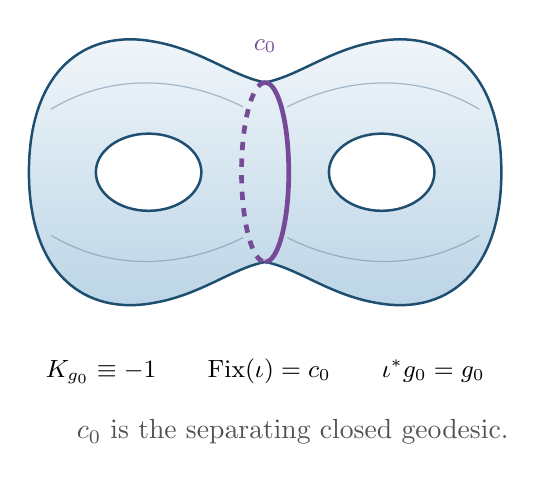
\begin{tikzpicture}
		\begin{scope}[scale=1]
			\path[surface]
			(-3.00,0).. controls (-3.00,1.30) and (-2.28,1.82).. (-1.42,1.66).. controls (-0.82,1.56) and (-0.42,1.22).. (0,1.14).. controls (0.42,1.22) and (0.82,1.56).. (1.42,1.66).. controls (2.28,1.82) and (3.00,1.30).. (3.00,0).. controls (3.00,-1.30) and (2.28,-1.82).. (1.42,-1.66).. controls (0.82,-1.56) and (0.42,-1.22).. (0,-1.14).. controls (-0.42,-1.22) and (-0.82,-1.56).. (-1.42,-1.66).. controls (-2.28,-1.82) and (-3.00,-1.30).. (-3.00,0)-- cycle;
			\path[fill=white, draw=surfaceedge, line width=0.9pt] (-1.48,0) ellipse (0.67 and 0.49);
			\path[fill=white, draw=surfaceedge, line width=0.9pt] (1.48,0) ellipse (0.67 and 0.49);
			\draw[contour] (-2.72,0.80)..controls (-1.92,1.28) and (-1.02,1.20).. (-0.28,0.83);
			\draw[contour] (2.72,0.80)..controls (1.92,1.28) and (1.02,1.20).. (0.28,0.83);
			\draw[contour] (-2.72,-0.80)..controls (-1.92,-1.28) and (-1.02,-1.20).. (-0.28,-0.83);
			\draw[contour] (2.72,-0.80)..controls (1.92,-1.28) and (1.02,-1.20).. ( 0.28,-0.83);
			\draw[seam, dashed] (0,1.14) arc[start angle=90,end angle=270,x radius=0.30,y radius=1.14];
			\draw[seam] (0,-1.14) arc[start angle=-90,end angle=90,x radius=0.30,y radius=1.14];
		\end{scope}

		\node[font=\small, text=glueboundary, fill=white, inner sep=1.5pt] at (0,1.6) {$c_{0}$};
		\node[font=\small] at (0,-2.53) {$K_{g_{0}}\equiv -1$\qquad $\operatorname{Fix}(\iota)=c_{0}$\qquad $\iota^{\ast}g_{0}=g_{0}$};

		\node[note] at (0.35,-3.3) {$c_0$ is the separating closed geodesic.};
	\end{tikzpicture}
\end{center}

Now choose a sufficiently small, $\iota$-invariant, tubular neighborhood $U$ containing $c_0$ and the local coordinate $U\simeq (-3a,3a)\times S^{1}$ where $a$ is some small constant. Assign the coordinate $(r,\theta)$ to the point in this trivialization with $\iota(r,\theta)=(-r,\theta)$. In particular, we have $c_0=\{(0,\theta)\mid \theta\in S^{1}\}$ in this coordinate.

Define function $s:\mathbb{R}\to\mathbb{R}$ by
\begin{equation}
	s(t)=\left\{
	\begin{aligned}
		 & \mathrm{e}^{-\frac{1}{t}},\qquad & t>0,     \\
		 & 0,\qquad                         & t\leq 0.
	\end{aligned}
	\right.
\end{equation}

This function $s$ is smooth with $s^{(j)}(0)=0$ for all $j\ge 0$.

Now we can define the cutoff function
\begin{equation}
	\begin{aligned}
		\eta:(-3a,3a) & \longrightarrow \mathbb{R} &                                                                  \\
		r             & \longmapsto \eta(r)        & \coloneq \dfrac{s(4a^2-r^2)}{s(4a^2-r^2)+s(r^2-\frac{9a^2}{4})}.
	\end{aligned}
\end{equation}

Easy to check that this cutoff function $\eta$ is smooth, constant $1$ for $|r|\le \frac{3a}{2}$ and $0$ for $|r|\geq 2a$. It takes values in $[0,1]$, and all derivatives of positive order vanish at the transition endpoints.

Lastly, define an even function $H:(-3a,3a)\to \mathbb{R}$ by
\begin{equation}
	H(r)=\left\{
	\begin{aligned}
		 & \mathrm{e}^{-\frac{a^2}{r^2}}\sin^{2}\left(\frac{a\pi}{r}\right),\qquad & r\neq 0, \\
		 & 0,\qquad                                                                & r=0.
	\end{aligned}
	\right.
\end{equation}

Clearly, $H\geq 0$. And $H(r)=0$ if and only if $r=0$ or $r=\frac{a}{n}$ for integer $n\neq 0$. Denote the zeros of $H$ by
\begin{displaymath}
	Z(H)=H^{-1}(0)=\{0\}\bigcup_{n=1}^{\infty}\{\frac{a}{n},-\frac{a}{n}\}.
\end{displaymath}

Next, we can compute the derivatives. When $r=0$, we have $H^{(n)}(0)=0$ for every integer $n\ge 0$, $H(r)$ is infinitely flat at $0$. For the other zeros $r_n=\frac{a}{n}$, we have
\begin{displaymath}
	H(r_n)=H'(r_n)=0;\qquad H''(r_n)=\frac{2\pi^2}{a^2} n^4\mathrm{e}^{-n^2}>0.
\end{displaymath}

Thus, $H$ is not infinitely flat at $r_n$ or $-r_n$.

Lastly, define a function $q:M\to \mathbb{R}$ by
\begin{displaymath}
	q(x)=\left\{
	\begin{aligned}
		 & \eta(r)H(r)+(1-\eta(r)),\qquad &  & x\in U,            \\
		 & 1,\qquad                       &  & x\in M\setminus U.
	\end{aligned}
	\right.
\end{displaymath}

Easy to check that, $q(x)$ is a smooth function on $M$ because near the boundary of the tubular $q\equiv1$. Moreover, we have $q\circ\iota=q$. We can compute that for $x=(r,\theta)\in U$,
\begin{displaymath}
	q(x)=q(r,\theta)=\left\{
	\begin{aligned}
		 & H(r),\qquad              &  & |r|\leq\frac{3a}{2},         \\
		 & 1+\eta(r)(H(r)-1),\qquad &  & \frac{3a}{2}\leq |r|\leq 2a, \\
		 & 1,\qquad                 &  & |r|\geq 2a.
	\end{aligned}
	\right.
\end{displaymath}

The set of zeros of $q(x)$ is given by circles:
\begin{displaymath}
	Z(q)=q^{-1}(0)=c_{0}\bigcup_{j=1}^{\infty}(c_{j}^{+}\cup c_{j}^{-}),\qquad c_{j}^{\pm}=\{(\pm\frac{a}{j},\theta)\mid \theta\in S^{1}\}.
\end{displaymath}

Note that $q$ is not constantly $0$ on $M$, by Kazdan-Warner Theorem (see~\cite{KazdanWarner1974}), there is a unique metric $g$ on $M$ such that the Gaussian curvature $K_{g}(x)=-q(x)$. In fact, there exists a unique smooth function $u$, such that
\begin{equation}
	\Delta_{g_0}u-K_{g_{0}}=\Delta_{g_0}u+1=q\mathrm{e}^{2u}.
\end{equation}

Let $g=\mathrm{e}^{2u}g_{0}$, we can compute
\begin{displaymath}
	K_{g}=\mathrm{e}^{-2u}(K_{g_{0}}-\Delta_{g_{0}}u)=e^{-2u}(-1-\Delta_{g_{0}}u)=-q.
\end{displaymath}

Since $\iota$ preserves both $g_{0}$ and $q$, the function $u\circ\iota$ satisfies the same equation as $u$. Uniqueness gives $u\circ\iota=u$, and hence $\iota^{\ast}g=g$. Therefore, the fixed-point set $c_0$ is a geodesic with respect to $g$. Since $K_{g}|_{c_0}=0$, it is a closed flat geodesic.

By Theorem~\ref{thm_2_1}, the geodesic flow of $g$ is not Anosov.

Next, we will verify $\area(F_{\infty}(g))=0$. By definition, we have
\begin{displaymath}
	F_{\infty}(g)=\{x\mid \nabla_{g}^{j}q(x)=0,\quad\forall j\ge 0\}\subset Z(q).
\end{displaymath}

On $c_{0}$, $r=0$, we know $q(0,\theta)=H(0)$ is infinitely flat, thus $c_{0}\subset F_{\infty}(g)$. But the other circles $c_{n}^{\pm}$, we have
\begin{displaymath}
	K_{g}(x)\vert_{x\in c_{n}^{\pm}}=-H(\pm\frac{a}{n})=0,\qquad \partial^2_{r}H(\pm\frac{a}{n})\neq 0.
\end{displaymath}

Therefore, we can conclude that $F_{\infty}(g)=c_0$, which has zero area. Thus, the geodesic flow is ergodic with respect to the Liouville measure.

Lastly, each annulus $(a/(n+1),a/n)\times S^1$ and its reflected counterpart is contained in $N$ and is bounded by zero-curvature circles. These annuli are distinct connected components of $N$. Hence, $N$ has infinitely many connected components.

\section{Ergodicity on Smooth Manifolds in Higher Dimensions}\label{sec5}
Throughout this section, we will work on smooth closed rank one manifold $(M,g)$ of nonpositive curvature. Let $\mu_L$ denote the normalized Liouville measure with $\mu_L(T^{1}M)=1$ and $\vol$ is the Riemannian volume of $M$. For any $x\in M$, let $\sigma_{x}$ be the smooth normalized rotationally invariant measure on the sphere $T^{1}_{x}M\simeq S^{n-1}$, so that $\sigma_{x}(T^{1}_{x}M)=1$. Choose $\bm{v}\in T^{1}_{x}M$, define the orthogonal complement of $\bm{v}$ as
\begin{displaymath}
	E_{\bm{v}}\coloneq\bm{v}^{\perp}=\left\{\bm{w}\in T_{x}M\mid \langle\bm{v},\bm{w}\rangle=0\right\}.
\end{displaymath}

For any $t\in\mathbb{R}$, let
\begin{displaymath}
	P_{\bm{v},t}:E_{\bm{v}}\longrightarrow E_{\phi_{t}(\bm{v})}
\end{displaymath}
be the parallel transport along the geodesic $c_{\bm{v}}$. Since the parallel transport along a fixed geodesic preserves the Riemannian inner product, this map is well-defined and a linear isometry.

By definition, the singular set can be written as
\begin{displaymath}
	\begin{aligned}
		\sing & =\left\{\bm{v}\in T^{1}M\mid \rank(\bm{v})\ge2\right\}                                                                                                         \\
		      & =\left\{\bm{v}\in T^{1}M\mid \exists 0\neq \bm{w}\in E_{\bm{v}},~R(P_{\bm{v},t}(\bm{w}),c'_{\bm{v}}(t))c'_{\bm{v}}(t)=0,\quad \forall t\in\mathbb{R} \right\}.
	\end{aligned}
\end{displaymath}

By the Pesin-Hopf argument, the geodesic flow is ergodic on the regular rank one set; therefore, if $\mu_L(\sing)=0$, it is ergodic on $T^{1}M$ with respect to the Liouville measure. See~\cite{BallmannBrin1982,Burns1983,BurnsMatveev2021, Pesin1977}. Our target is to prove the singular set has zero Liouville measure. Start with the curvature Jacobi operator:

\begin{definition}[Curvature Jacobi Operator]\label{def_5_1}
	For any $x\in M$ and $\bm{0}\neq\bm{v}\in T_{x}M$, let $J_{\bm{v}}:T_{x}M \to T_{x}M$ denote the Curvature Jacobi Operator defined by
	\begin{displaymath}
		J_{\bm{v}}(\bm{w})=-R(\bm{w},\bm{v})\bm{v}.
	\end{displaymath}
\end{definition}

Restricting the operator to $E_{\bm{v}}$ for the given $\bm{v}\neq 0$, we can also define the Reduced Jacobi Operator as

\begin{definition}[Reduced Jacobi Operator]\label{def_5_2}
	For any $x\in M$ and $\bm{v}\in T^{1}_{x}M$, we define the Reduced Normal Jacobi Operator as
	\begin{displaymath}
		\begin{aligned}
			J^{\perp}_{\bm{v}}: & E_{\bm{v}} & \longrightarrow & ~~E_{\bm{v}}             \\
			                    & \bm{w}     & \longmapsto     & -R(\bm{w},\bm{v})\bm{v}.
		\end{aligned}
	\end{displaymath}
\end{definition}

For convenience, our definitions~\ref{def_5_1} and~\ref{def_5_2} differ from the classical ones by a sign. More discussions of these operators can be found in~\cite{BlazicGilkeyNikcevicSimon2006,Gilkey2001}.

\begin{proposition}
	The curvature Jacobi operator and reduced Jacobi operator have the following properties:
	\begin{enumerate}
		\item $J_{\bm{v}}$ is linear and self-adjoint, so is $J^{\perp}_{\bm{v}}$.
		\item $J_{\bm{v}}(\bm{v})=0$. $\bm{v}$ is an eigenvector to $0$.
		\item $J_{\bm{v}}(E_{\bm{v}})\subset E_{\bm{v}}$, thus, the reduced Jacobi operator is well-defined.
		\item $J^{\perp}_{\bm{v}}$ is positive semidefinite if $(M,g)$ has nonpositive sectional curvature.
	\end{enumerate}
\end{proposition}

\begin{proof}
	Linearity follows from the Riemannian curvature tensor. For any $\bm{u},\bm{w}\in T_{x}M$, we can compute
	\begin{displaymath}
		\langle J_{\bm{v}}(\bm{w}),\bm{u}\rangle=-\langle R(\bm{w},\bm{v})\bm{v},\bm{u}\rangle=-\langle R(\bm{u},\bm{v})\bm{v},\bm{w}\rangle= \langle J_{\bm{v}}(\bm{u}),\bm{w}\rangle.
	\end{displaymath}

	Hence, $J^{\ast}_{\bm{v}}=J_{\bm{v}}$. $J_{\bm{v}}(\bm{v})=0$ is clear from the definition.

	For any $\bm{w}\in E_{\bm{v}}$, we have
	\begin{displaymath}
		\langle J_{\bm{v}}(\bm{w}),\bm{v}\rangle=-\langle R(\bm{w},\bm{v})\bm{v},\bm{v}\rangle=0.
	\end{displaymath}

	Thus, $J_{\bm{v}}(\bm{w})\in E_{\bm{v}}$. The restriction $J^{\perp}$ is well-defined.

	Lastly, for any unit vector $\bm{w}\in E_{\bm{v}}$, we have
	\begin{displaymath}
		\langle J^{\perp}_{\bm{v}}(\bm{w}),\bm{w}\rangle=-\langle R(\bm{w},\bm{v})\bm{v},\bm{w}\rangle=-K(\bm{v},\bm{w}).
	\end{displaymath}

	This is the negative of the sectional curvature, hence, it is positive semidefinite given $(M,g)$ has nonpositive sectional curvature.
\end{proof}

\begin{definition}[Reduced Jacobi Curvature Determinant]\label{def_5_3}
	For given $x$ and $\bm{v}\in T^{1}_{x}M$, we denote the determinant of $J^{\perp}_{\bm{v}}$ by
	\begin{displaymath}
		\begin{aligned}
			q_{J}: & T^{1}M     & \longrightarrow & \mathbb{R}                \\
			       & (x,\bm{v}) & \longmapsto     & \det(J^{\perp}_{\bm{v}}).
		\end{aligned}
	\end{displaymath}

	On manifolds of nonpositive curvature, we can see that $q_{J}\geq 0$.
\end{definition}

Note that $J^{\perp}_{\bm{v}}$ is self-adjoint, we can choose an orthonormal eigenbasis $\{\bm{e}_1,\ldots,\bm{e}_{n-1}\}$ of $E_{\bm{v}}$. Denote the sectional curvature by
\begin{displaymath}
	\kappa_{i}=-\langle J^{\perp}_{\bm{v}}(\bm{e}_i),\bm{e}_i\rangle=\langle R(\bm{e}_i,\bm{v})\bm{v},\bm{e}_i\rangle,
\end{displaymath}
which is the sectional curvature of $\bm{v}$ and $\bm{e}_i$. We can compute
\begin{equation}
	q_J(x,\bm{v})=\prod_{i=1}^{n-1}(-\kappa_{i}).
\end{equation}

By definition, we have
\begin{displaymath}
	q_{J}(x,\bm{v})=0 \Leftrightarrow\ker J^{\perp}_{\bm{v}}\neq \{0\}\Leftrightarrow \exists \bm{0}\neq\bm{w}\in E_{\bm{v}},~J^{\perp}_{\bm{v}}(\bm{w})=\bm{0}.
\end{displaymath}

\begin{lemma}\label{lem_5_1}
	Fix $x\in M$ and a local frame near $x$, denote $q_{J}^{x}=q_J(x,\cdot):T^{1}_{x}M\to \mathbb{R}$.
	\begin{displaymath}
		q_{J}^{x}(\bm{v})=\det(J_{\bm{v}}^{\perp}).
	\end{displaymath}

	Then $q_{J}^{x}$ is the restriction to $T^{1}_{x}M\simeq S^{n-1}$ of a homogeneous polynomial of degree $2(n-1)$ in the component of $\bm{v}$.
\end{lemma}

\begin{proof}
	Choose a smooth orthonormal frame $\{\bm{e}_1(y),\ldots\bm{e}_n(y)\}$ for $y\in U$ in a small neighborhood $U$ of $x$. In $T_{x}M$, we use the basis $\{\bm{e}_1(x),\dots,\bm{e}_{n}(x)\}$ and write
	\begin{displaymath}
		J_{\bm{v}}={(a_{ij}(x,\bm{v}))}_{n\times n}.
	\end{displaymath}
	This is an $n\times n$ matrix with elements $a_{ij}(x,\bm{v})$ being smooth functions of $\bm{v}$. Write $\bm{v}=\sum_{k=1}^n v_k\bm{e}_{k}(x)$, we have

	\begin{displaymath}
		\begin{aligned}
			a_{ij}(x,\bm{v}) & =\langle J_{\bm{v}}(\bm{e}_j(x)),\bm{e}_{i}(x) \rangle                                                        \\
			                 & =-\langle R(\bm{e}_{j}(x),\bm{v})\bm{v},\bm{e}_{i}(x)\rangle                                                  \\
			                 & =-\langle R(\bm{e}_{j}(x),\sum_{k=1}^n v_k\bm{e}_{k}(x))(\sum_{l=1}^{n}v_l\bm{e}_{l}(x)),\bm{e}_{i}(x)\rangle \\
			                 & =-\sum_{k,l=1}^{n} v_k v_l\langle R(\bm{e}_{j}(x),\bm{e}_{k}(x))\bm{e}_{l}(x),\bm{e}_{i}(x)\rangle.
		\end{aligned}
	\end{displaymath}

	Once we fix $x$ and the frame, the curvature component are independent of $\bm{v}$. We can see that $a_{ij}(x,\bm{v})$ is a homogeneous polynomial of degree $2$ in terms of $v_k$'s.

	Claim that
	\begin{equation}
		q_{J}^{x}(\bm{v})=\det (J_{\bm{v}}^{\perp})=\operatorname{tr}(\bigwedge^{n-1}J_{\bm{v}})=\sigma_{n-1}(J_{\bm{v}}).
	\end{equation}

	Here $\sigma_{n-1}(J_{\bm{v}})$ is the $(n-1)$-th elementary symmetric polynomials defined in
	\begin{displaymath}
		\det(J_{\bm{v}}+t I)=t^n+\sigma_1(J_{\bm{v}})t^{n-1}+\cdots+\sigma_{n-1}(J_{\bm{v}})t+\det(J_{\bm{v}}).
	\end{displaymath}

	Note that $J_{\bm{v}}(\bm{v})=0$, we have the invariant decomposition $J_{\bm{v}}=0\oplus J^{\perp}_{\bm{v}}$ on $T_{x}M=\mathbb{R}\bm{v}\oplus E_{\bm{v}}$, thus, in $\sigma_{n-1}(J_{\bm{v}})$, all terms vanish except the product of the other $n-1$ eigenvalues of $J_{\bm{v}}$, which is exactly our $\det(J^{\perp}_{\bm{v}})$. Because each element in the matrix is a homogeneous polynomial of degree $2$ in terms of $v_{k}$'s, the corresponding $\sigma_{n-1}(J_{\bm{v}})$ is a homogeneous polynomial of degree $2(n-1)$ restricted on the sphere.
\end{proof}

\begin{definition}[Fiberwise Second Moment of the Reduced Jacobi Determinant]
	Define a function $h_J:M\to\mathbb{R}$ by
	\begin{displaymath}
		h_{J}(x)=\int_{T^{1}_{x}M}q_{J}^{2}(x,\bm{v})\,\mathrm{d}\sigma_{x}(\bm{v}).
	\end{displaymath}

	Clearly, $h_{J}$ is smooth, non-negative. $h_{J}(x)=0$ if and only if $q_{J}(x,\cdot)$ is constantly $0$ on $T^{1}_{x}M$.
\end{definition}

Now we will define the analogous set, denoted by $F^{J}_{\infty}$ to the infinite flat set $F_{\infty}$ (Definition~\ref{def_2_1}) as in the case of dimension $2$.

\begin{definition}
	On $M$ we define two sets:
	\begin{enumerate}
		\item The set of degenerate points $\mathcal{D}\coloneq h_{J}^{-1}(0)=\{x\in M\mid q_{J}^{x}\equiv 0\}$.
		\item The Infinite-order Vanishing Set of $h_{J}$:
		      \begin{displaymath}
			      F_{\infty}^{J}\coloneq\{x\in M\mid {(\nabla^{k}h_{J})}_{x}=0,\quad \forall k=0,1,\ldots\}.
		      \end{displaymath}
	\end{enumerate}
\end{definition}

As we computed in the proof of Lemma~\ref{lem_3_2}, for point $x\in F^{J}_{\infty}$, one can check for any multi-index $\alpha\in\mathbb{N}^{n}$, $\partial^{\alpha}h_{J}(x)=0$ for any $|\alpha|\ge 0$ in any local chart.

This definition coincide with $F_{\infty}$ on surface, on which $q_{J}(x,\bm{v})=-K(x)$ and thus, $h_{J}(x)={K(x)}^2$. At this time, $F^{J}_{\infty}=F_{\infty}$.

\begin{lemma}\label{lem_5_2}
	The set of zeros of finite-order of the smooth function $h_{J}$, denoted by $\mathcal{D}\setminus F^{J}_{\infty}$ can be covered by countably many hypersurfaces of dimension $n-1$. Thus, $\vol(\mathcal{D}\setminus F^{J}_{\infty})=0$.
\end{lemma}

\begin{proof}
	Choose a countable coordinate atlas $(U_{j},\psi_{j})$ covers $M$. In each chart $U_{j}$ and for each multi-index $\beta$, consider
	\begin{displaymath}
		H_{j,\beta}=\left\{y\in U_{j}\mid \partial^\beta h_J(y)=0,\; d{(\partial^\beta h_J)}_y\ne0\right\}.
	\end{displaymath}
	By the Implicit Function Theorem, for any point $p\in H_{j,\beta}$, we can find a sufficiently small neighborhood $V_{p}\subset U_{j}$ of it, such that
	\begin{displaymath}
		H_{j,\beta}\cap V_{p}={(\partial^{\beta}h_{J})}^{-1}(0) \cap V_{p}
	\end{displaymath}
	is a smooth hypersurface. Note that $U_j$ is second countable, hence the relative open cover $H_{j,\beta}\cap V_{p}$ for all $p\in H_{j,\beta}$ has a countable open cover.

	Now in some $U_{j}$, choose $x\in \mathcal{D}\setminus F_\infty^J$, choose a derivative $\partial^{\alpha} h_J(x)\ne0$ of minimal order. Select $i$ with $\alpha_{i}>0$ and set $\beta=\alpha-e_{i}$. Then
	\begin{displaymath}
		\partial^\beta h_J(x)=0,\qquad \partial_{i}\partial^{\beta} h_J(x)\ne0.
	\end{displaymath}

	Thus, $x\in H_{j,\beta}$. Therefore, this set $\mathcal{D}\setminus F^{J}_{\infty}$ is contained in the union of all possible $H_{j,\beta}$, each of which is covered by a collection of countably many hypersurfaces. Since $j$ and the multi-indices $\beta$ are countable, the countable cover of $\mathcal{D}\setminus F^{J}_{\infty}$ follows, leading to that
	\begin{displaymath}
		\vol(\mathcal{D}\setminus F^{J}_{\infty})=0.
	\end{displaymath}

	Equivalently, we can see that $\vol(\mathcal{D})=\vol(F^{J}_{\infty})$.
\end{proof}

\begin{remark}
	This result actually holds for any smooth function $f(x)$ defined on a smooth manifold of dimension $n$. On surfaces, we have $\area(F_{\infty})=\area (\{x\mid K(x)=0\})$.
\end{remark}

\begin{lemma}\label{lem_5_3}
	If $x\notin \mathcal{D}$, we have $q_J(x,\cdot):T^{1}_{x}M\to\mathbb{R}$ is not constantly $0$, and
	\begin{displaymath}
		\sigma_{x}\left( \left\{\bm{v}\in T^{1}_{x}M\mid q_{J}(x,\bm{v})=0\right\} \right)=0.
	\end{displaymath}
\end{lemma}
This is the generalization of Lemma~\ref{lem_3_2} to higher dimensional fibers.

\begin{proof}
	Fix $x$ and some local chart $(U,\psi)$. By Lemma~\ref{lem_5_1}, $q_{J}^{x}$ is a nonzero homogeneous polynomial of degree $2(n-1)$ with constant coefficients (only depends on $x$) restricted on the sphere $S^{n-1}$. Denote the polynomial by $P$ and the set of zeros of $P$ in $T_{x}M\simeq \mathbb{R}^{n}$ by $Z(P)$.

	By the homogeneity of $q_{J}^{x}$, if a point $\omega\in S^{n-1}$ is a zero point, then the entire line passing through the origin and $\omega$ is also contained in the zero points set. By switching to hyperspherical coordinate and use the Fubini's theorem, we have the Lebesgue measure of $Z(P)$ in $\mathbb{R}^n$ can be computed by
	\begin{displaymath}
		0=\operatorname{Leb}(Z(P))=\omega_{n-1}\int_0^{\infty} t^{n-1}\sigma_x(Z(P)\cap S^{n-1})\,\mathrm{d}t.
	\end{displaymath}
	It is a standard fact that the set of zeros of a nonzero multivariate polynomial on $\mathbb{R}^{n}$ has Lebesgue measure zero. Therefore, the set of zeros of $q_{J}(x,\cdot)$ on $T^{1}_{x}M$ has measure zero.
\end{proof}

\begin{lemma}\label{lem_5_4}
	Suppose $\bm{v}\in T^{1}_{x}M$ is singular, then $q_J(x,\bm{v})=0$.
\end{lemma}

\begin{proof}
	By definition, $\bm{v}$ is singular, we can find a nonzero parallel normal Jacobi field $Y$ with $\bm{w}=Y(0)$. Then, $J^{\perp}_{\bm{v}}(\bm{w})=0$, $\ker J^{\perp}_{\bm{v}}$ is non-trivial, $q_J(x,\bm{v})=0$.
\end{proof}

We are ready to prove Theorem~\ref{thm_2_4}:

\manifold*

\begin{proof}
	By Lemma~\ref{lem_5_4}, $\sing$ is a subset of the set of zeros $Z(q_{J})$ of $q_J$. Therefore, we have
	\begin{displaymath}
		\begin{aligned}
			\mu_{L}(\sing) & \leq \mu_{L}(Z(q_{J}))                                                                                                                   \\
			               & =\dfrac{1}{\vol(M)}\int_{M}\sigma_{x}(Z(q_{J})\cap T^{1}_{x}M)\,\mathrm{d}\vol(x)                                                        \\
			               & =\dfrac{1}{\vol(M)}\left(\int_{\mathcal{D}}+\int_{M\setminus \mathcal{D}}\right) \sigma_{x}(Z(q_{J})\cap T^{1}_{x}M)\,\mathrm{d}\vol(x).
		\end{aligned}
	\end{displaymath}

	By Lemma~\ref{lem_5_3}, for any $x\in M\setminus \mathcal{D}$, $\sigma_{x}(Z(q_{J})\cap T^{1}_{x}M)=0$, thus the integration is also $0$. For $x\in \mathcal{D}$, we have $q_{J}(x,\cdot)=0$ on the whole $T^{1}_{x}M$, with the fiber measure of the set of zero $\sigma_{x}(Z(q_{J})\cap T^{1}_{x}M)=1$. Combine them together, we obtain that
	\begin{displaymath}
		\mu_{L}(\sing)\le \dfrac{1}{\vol(M)}\int_{\mathcal{D}}1\,\mathrm{d}\vol(x)=\dfrac{\vol(\mathcal{D})}{\vol(M)}.
	\end{displaymath}

	By Lemma~\ref{lem_5_2}, $\vol(\mathcal{D}\setminus F^{J}_{\infty})=0$. Therefore, we have
	\begin{displaymath}
		\mu_{L}(\sing)\leq\dfrac{\vol(F^{J}_{\infty})}{\vol(M)}.
	\end{displaymath}

	In particular, if $F^{J}_{\infty}$ has zero measure, then the geodesic flow is ergodic.
\end{proof}

\section{Ergodicity on Real Analytic Rank One Manifolds}\label{sec6}
We now prove Theorem~\ref{thm_2_5} in the real analytic setting.

\analymlfd*

Again, our target is to show the singular set has zero Liouville measure. Similar notations as in~\ref{sec5} will be used. Let $x\in M$ and $\bm{v}\in T^{1}_{x}M$, recall $E_{\bm{v}}$ denote the orthogonal complement of $\bm{v}$ and $P_{\bm{v},t}:E_{\bm{v}}\to E_{\phi_{t}(\bm{v})}$ denote the parallel transport along $c_{\bm{v}}$.

\begin{definition}\label{def_6_1}
	On $E_{\bm{v}}$ we define the parallel-transport pullback of the curvature endomorphism $A(\bm{v},t):E_{\bm{v}}\to E_{\bm{v}}$ by
	\begin{equation}
		A(\bm{v},t)(\bm{w})=P^{-1}_{\bm{v},t}\circ R(P_{\bm{v},t}(\bm{w}),c'_{\bm{v}}(t))c'_{\bm{v}}(t).
	\end{equation}

	Then, $A(\bm{v},t)$ is a self-adjoint linear operator.
\end{definition}

\begin{proof}
	We first show that this operator is well-defined. Fix $\bm{v}$ and choose $\bm{w}\in E_{\bm{v}}$, we need to show $A(\bm{v},t)(\bm{w})\in E_{\bm{v}}$ as well. Denote $\bm{w}_t=P_{\bm{v},t}\bm{w}$, the curvature symmetries imply
	\begin{displaymath}
		\langle R(\bm{w}_t,c'_{\bm{v}}(t))c'_{\bm{v}}(t),c'_{\bm{v}}(t)\rangle=0.
	\end{displaymath}
	Thus, the curvature vector lies in $E_{\phi_{t}(\bm{v})}$, so $A(\bm{v},t)$ is well-defined.

	Linearity follows immediately from the fact that $P_{\bm{v},t}$, its inverse, and the curvature endomorphism are all linear maps. To verify that it is self-adjoint, choose $\bm{u},\bm{w}\in E_{\bm{v}}$ and denote $\bm{u}_t=P_{\bm{v},t}(\bm{u})$ and $\bm{w}_t=P_{\bm{v},t}(\bm{w})$.

	\begin{displaymath}
		\begin{aligned}
			\langle A(\bm{v},t)(\bm{u}),\bm{w}\rangle & =\langle P^{-1}_{\bm{v},t}\circ R(\bm{u}_t,c'_{\bm{v}}(t))c'_{\bm{v}}(t),\bm{w}\rangle \\
			                                          & =\langle R(\bm{u}_t,c'_{\bm{v}}(t))c'_{\bm{v}}(t),\bm{w}_{t}\rangle                    \\
			                                          & =R(\bm{u}_t, c'_{\bm{v}}(t),c'_{\bm{v}}(t),\bm{w}_t)                                   \\
			                                          & =R(\bm{w}_t,c'_{\bm{v}}(t),c'_{\bm{v}}(t),\bm{u}_t)                                    \\
			                                          & =\langle A(\bm{v},t)\bm{w},\bm{u}\rangle.
		\end{aligned}
	\end{displaymath}

	Therefore, $A^{\ast}(\bm{v},t)=A(\bm{v},t)$ is self-adjoint.
\end{proof}

\begin{definition}\label{def_6_2}
	For any $\bm{v}\in T^{1}M$, define the operator $Q(\bm{v}):E_{\bm{v}}\to E_{\bm{v}}$ by
	\begin{displaymath}
		Q(\bm{v})(\bm{w})=\int_{-1}^{1} A^{\ast}(\bm{v},t)\circ A(\bm{v},t)(\bm{w})\,\mathrm{d}t.
	\end{displaymath}

	Then, $Q(\bm{v})$ is self-adjoint and positive semidefinite.
\end{definition}

\begin{proof}
	Choose any $\bm{w}\in E_{\bm{v}}$. We can see that $Q(\bm{v})$ is well-defined from $E_{\bm{v}}$ to itself. This is because $A(\bm{v},t)$ preserves $E_{\bm{v}}$, so does $A^{\ast}(\bm{v},t)\circ A(\bm{v},t)$. This holds for any $t\in (-1,1)$ and hence, the integral also lies in $E_{\bm{v}}$. $A^{\ast}(\bm{v},t)A(\bm{v},t)$ is self-adjoint for all $t$, so is $Q(\bm{v})$. To show that it is positive semidefinite,

	\begin{displaymath}
		\begin{aligned}
			\langle Q(\bm{v})(\bm{w}),\bm{w}\rangle & =\langle \int_{-1}^{1} A^{\ast}(\bm{v},t)\circ A(\bm{v},t)(\bm{w})\,\mathrm{d}t,\bm{w}\rangle \\
			                                        & =\int_{-1}^{1}\langle A^{\ast}(\bm{v},t)\circ A(\bm{v},t)(\bm{w}),\bm{w}\rangle\,\mathrm{d}t  \\
			                                        & =\int_{-1}^{1}\langle A(\bm{v},t)(\bm{w}),A(\bm{v},t)(\bm{w})\rangle\,\mathrm{d}t             \\
			                                        & =\int_{-1}^{1}{\lVert A(\bm{v},t)(\bm{w})\rVert}^2\,\mathrm{d}t\geq 0.
		\end{aligned}
	\end{displaymath}
\end{proof}

\begin{definition}\label{def_6_3}
	Define the function $D:T^{1}M\to\mathbb{R}$ by
	\begin{equation}
		D(\bm{v})\coloneq \det Q(\bm{v}).
	\end{equation}

	From Definition~\ref{def_6_2}, we have $Q(\bm{v})$ positive semidefinite, thus, $D(\bm{v})\ge 0$.
\end{definition}

One important property is that in real analytic setting, the set of zeros of $D$ defined in Definition~\ref{def_6_3} characterize the singular set of $T^{1}M$.

\begin{theorem}\label{thm_6_1}
	A vector $\bm v\in T^1M$ is singular if and only if $D(\bm{v})=0$.
\end{theorem}

\begin{proof}
	Suppose that $\bm{v}$ lies in the singular set, $\rank(\bm{v})\ge 2$. By the definition of rank, we can find a nonzero parallel normal Jacobi field $Y$ along $c_{\bm{v}}$. Denote $\bm{w}=Y(0)\in E_{\bm{v}}$ which is a nonzero vector and $Y(t)=P_{\bm{v},t}(\bm{w})$.

	$Y(t)$ should satisfy the Jacobi equation, that is
	\begin{displaymath}
		\dfrac{\mathrm{D}^2 Y}{\mathrm{d}t^{2}}+R(Y(t),c'_{\bm{v}}(t))c'_{\bm{v}}(t)=0.
	\end{displaymath}

	Since $Y(t)$ is the parallel vector field, $\dfrac{\mathrm{D}Y}{\mathrm{d}t}(t)=0$, thus, $\dfrac{\mathrm{D}^{2}Y}{\mathrm{d}t^2}(t)=0$. Therefore, we get
	\begin{displaymath}
		R(Y(t),c'_{\bm{v}}(t))c'_{\bm{v}}(t)=0.
	\end{displaymath}

	Hence,
	\begin{displaymath}
		A(\bm{v},t)(\bm{w})=P^{-1}_{\bm{v},t}\circ R(P_{\bm{v},t}(\bm{w}),c'_{\bm{v}}(t))c'_{\bm{v}}(t)=0,
	\end{displaymath}
	$Q(\bm{v})(\bm{w})=0$ and $D(\bm{v})=0$.

	Conversely, suppose that $D(\bm{v})=0$, then $\ker Q(\bm{v})$ is non-trivial. Choose a nonzero vector $\bm{w}\in \ker Q(\bm{v})\subset E_{\bm{v}}$, we have
	\begin{displaymath}
		0=\langle Q(\bm{v})(\bm{w}),\bm{w}\rangle=\int_{-1}^{1} {\lVert A(\bm{v},t)(\bm{w})\rVert}^{2}\,\mathrm{d}t.
	\end{displaymath}

	$A(\bm{v},t)(\bm{w})$ is continuous, this implies $A(\bm{v},t)(\bm{w})=0$ for $t\in (-1,1)$. Since the metric is real analytic, geodesics and parallel transport depend real analytically on time. Thus, $t\mapsto A(\bm{v},t)\bm{w}$ is real analytic on $\mathbb{R}$. By the unique continuation of the analytic function, we get
	\begin{displaymath}
		A(\bm{v},t)(\bm{w})=0,\qquad t\in\mathbb{R}.
	\end{displaymath}

	Now let $Y(t)=P_{\bm{v},t}(\bm{w})$, from the above argument, we have
	\begin{displaymath}
		R(Y(t),c'_{\bm{v}}(t))c'_{\bm{v}}(t)=0,\qquad t\in\mathbb{R}.
	\end{displaymath}

	Together with $Y(t)$ is parallel, the second order derivative is also zero. $Y(t)$ satisfies the Jacobi equation, which is a nonzero parallel normal Jacobi field along $c_{\bm{v}}$. Thus, $\rank(\bm{v})\ge 2$, $\bm{v}\in\sing$.
\end{proof}

Furthermore, we can evaluate the rank of the vector $\bm{v}$ by study the operator $Q(\bm{v})$.

\begin{corollary}
	In the setting of real analytic metric,
	\begin{displaymath}
		\rank(\bm{v})=1+\dim\ker Q(\bm{v}).
	\end{displaymath}
\end{corollary}

We are ready to prove the Theorem~\ref{thm_2_5} now.

\begin{proof}[Proof of Theorem~\ref{thm_2_5}]
	In local real analytic frames of the normal bundle, the matrix entries of $A(\bm{v},t)$ are jointly real analytic in $(\bm{v},t)$. Integration over the fixed interval $(-1,1)$ therefore yields a real analytic endomorphism $Q$. Consequently, $D=\det Q$ is a globally defined real analytic function on $T^{1}M$.
	Given $\rank(M)=1$, we can find some $\bm{v}\in T^{1}M$ with rank $1$. By Theorem~\ref{thm_6_1}, $D(\bm{v})>0$, $D$ is not identically zero.

	Since the metric is analytic, the function $D:T^{1}M\to \mathbb{R}$ is real analytic. Thus, the set of zeros of $D$ on $T^1 M$ is a proper analytic subset, which has zero Liouville measure. Following from Theorem~\ref{thm_6_1},
	\begin{displaymath}
		\mu_{L}(\sing)=\mu_{L}(D^{-1}(0))=0,
	\end{displaymath}
	ergodicity of the geodesic flow follows.
\end{proof}

\begin{remark}
	If we only assume $C^{\infty}$-smoothness, what we can show is the singular set $\Lambda$ is a subset of the set of zeros $D^{-1}(0)$. The set of zeros of a smooth function may have positive measure, thus, this method cannot be applied to smooth manifolds directly.
\end{remark}

\section*{Acknowledgments}
The authors wish to express their gratitude to Professor Lan Wen for his guidance and support during our time working and studying at Peking University.

Fei Liu is partially supported by Natural Science Foundation of China under Grant No.~12571179.

Xiaokai Liu would love to thank Professor Raul Ures and Professor Jana Hertz for their invaluable guidance and continuous support at Southern University of Science and Technology.

\noindent{\bfseries Declaration of Interest:} The authors declare that they have no conflicts of interest.

\newpage
\printbibliography

\end{document}
